\documentclass{article}

% if you need to pass options to natbib, use, e.g.:
\PassOptionsToPackage{sort&compress, numbers}{natbib}
% before loading nips_2018

% ready for submission
\usepackage[final]{nips_2018}

% to compile a preprint version, e.g., for submission to arXiv, add
% add the [preprint] option:
% \usepackage[preprint]{nips_2018}

% to compile a camera-ready version, add the [final] option, e.g.:
% \usepackage[final]{nips_2018}

% to avoid loading the natbib package, add option nonatbib:
% \usepackage[nonatbib]{nips_2018}

\usepackage[utf8]{inputenc} % allow utf-8 input
\usepackage[T1]{fontenc}    % use 8-bit T1 fonts
\usepackage{booktabs}       % professional-quality tables
\usepackage{amsfonts}       % blackboard math symbols
\usepackage{nicefrac}       % compact symbols for 1/2, etc.
\usepackage{microtype}      % microtypography

\usepackage{mathrsfs}
\usepackage{graphicx}
\usepackage{xr-hyper} % cross-references (between documents)
\usepackage{xcolor} % Allow colors to be defined
\usepackage{geometry} % Used to adjust the document margins
\usepackage{amsmath} % Equations
\usepackage{amssymb} % Equations
% The hyperref package gives us a pdf with properly built
% internal navigation ('pdf bookmarks' for the table of contents,
% internal cross-reference links, web links for URLs, etc.)
\usepackage[hyphens]{url}
\usepackage[hypertexnames=false]{hyperref}
\usepackage[title,toc]{appendix}
\usepackage{natbib}
\usepackage{bm}
\usepackage{mathtools}
\usepackage{rotating,tabularx}

% Nicer default font (+ math font) than Computer Modern for most use cases
\usepackage{mathrsfs}
\usepackage{graphicx}
\usepackage{xr-hyper} % cross-references (between documents)
\usepackage{xcolor} % Allow colors to be defined
\usepackage{geometry} % Used to adjust the document margins
\usepackage{amsmath} % Equations
\usepackage{amssymb} % Equations
% Colors for the hyperref package
% The hyperref package gives us a pdf with properly built
% internal navigation ('pdf bookmarks' for the table of contents,
% internal cross-reference links, web links for URLs, etc.)
\usepackage{hyperref}
\usepackage[title,toc]{appendix}
\hypersetup{
    colorlinks=true,
    pdfborder=0 0 1,
    pdftitle=\georddtitle{},
    allcolors=[rgb]{0.00,0.38,0.59},
    allbordercolors=[rgb]{0.60,0.76,0.86}
}
\usepackage{natbib}
\usepackage{bm}
\usepackage{mathtools}
\usepackage{pdflscape}
\usepackage[doublespacing,nodisplayskipstretch]{setspace}
% only use if doublespacing:
\renewcommand*{\arraystretch}{0.8} % https://tex.stackexchange.com/questions/183562/how-to-reduce-vertical-space-in-matrix
\def\SmallColSep{\setlength{\arraycolsep}{3pt}}
% \usepackage{authblk}

\usepackage{enumitem}
\newlist{flatlist}{enumerate*}{1}
\setlist[flatlist]{label=(\arabic*)}


\newcommand{\mathbold}[1]{\bm{#1}} % if not using mathpazo

\DeclarePairedDelimiter{\parenthesis}{\lparen}{\rparen}
\DeclarePairedDelimiter{\squarebracket}{\lbrack}{\rbrack}
\DeclarePairedDelimiter{\curlybracket}{\lbrace}{\rbrace}
\DeclarePairedDelimiter{\absolutevalue}{\lvert}{\rvert}
\newcommand{\del}[1]{\parenthesis*{#1}}
\newcommand{\sbr}[1]{\squarebracket*{#1}}
\newcommand{\cbr}[1]{\curlybracket*{#1}}
\newcommand{\abs}[1]{\absolutevalue*{#1}}
% \DeclareMathOperator{\dif}{d}
\newcommand*{\diffdchar}{d}
\newcommand*{\dif}[1]{\mathop{\diffdchar #1}}
\DeclareMathOperator*{\argmin}{arg\,min}
\DeclareMathOperator*{\argmax}{arg\,max}
\let\Pr\relax
\DeclareMathOperator{\Pr}{\mathbb{P}}
\DeclareMathOperator{\E}{\mathbb{E}}
\DeclareMathOperator{\V}{\mathbb{V}}
\DeclareMathOperator{\cov}{{Cov}}
\DeclareMathOperator{\var}{{var}}
\DeclareMathOperator{\Ind}{\mathbb{I}}
\DeclareMathOperator*{\sgn}{{sgn}}

\DeclareMathOperator{\normal}{\mathcal{N}}
\DeclareMathOperator{\unif}{Uniform}
\DeclareMathOperator{\invchi}{\mathrm{Inv-\chi}^2}
\DeclareMathOperator{\ones}{\mathbf{1}}
\DeclareMathOperator{\GP}{\mathcal{GP}}
\newcommand{\building}{\mathtt{BuildClass}}
\newcommand{\district}{\mathtt{Distr}}

% \newcommand*{\trans}{^{\intercal}}
\newcommand*{\trans}{^{\top}}

\newcommand*{\area}{\mathcal{A}}
\newcommand*{\treat}{\mathrm{T}}
\newcommand*{\ctrol}{\mathrm{C}}
\newcommand*{\treatind}{Z}
\newcommand*{\treatarea}{\area{}^{\treat}}
\newcommand*{\ctrolarea}{\area{}^{\ctrol}}

\newcommand*{\sigmaf}{\sigma_{\mathrm{GP}}}
\newcommand*{\sigman}{\sigma_{\epsilon}}
\newcommand*{\sigmabeta}{\sigma_{\beta}}
\newcommand*{\sigmamu}{\sigma_{\mu}}
\newcommand*{\svec}{\mathbold{s}}
\newcommand*{\dvec}{\mathbold{d}}
\newcommand*{\wvec}{\mathbold{w}}
\newcommand*{\yvec}{\mathbold{y}}
\newcommand*{\Yvec}{\mathbold{Y}}
\newcommand*{\yt}{\Yvec_{\treat}}
\newcommand*{\yc}{\Yvec_{\ctrol}}
\newcommand*{\vvec}{\mathbold{v}}
\newcommand*{\muvec}{\mathbold{\mu}}
\newcommand*{\betavec}{\mathbold{\beta}}
\newcommand*{\residvec}{\mathbold{R}}
\newcommand*{\indep}{\protect\mathpalette{\protect\independenT}{\perp}}
\def\independenT#1#2{\mathrel{\rlap{$#1#2$}\mkern2mu{#1#2}}}
\newcommand*{\iid}{iid}
\newcommand*{\vectreat}{\Ind_{T}}

\newcommand*{\border}{\mathcal{B}}
\newcommand*{\sentinel}{\mathbold{b}}
\newcommand*{\numsent}{R}
\newcommand*{\sentinels}{\sentinel_{1:\numsent}}
\newcommand*{\isent}{r}
\newcommand*{\sentinelset}{\cbr{\sentinel_1,\ldots,\sentinel_\numsent}}

\newcommand*{\eye}{\mathbf{I}}

\DeclareMathOperator{\trace}{trace}
\newcommand*{\tauw}{\tau^{w}}
\newcommand*{\unifavg}{\tau^{\mathrm{UNIF}}}
\newcommand*{\invvar}{\tau^{\mathrm{INV}}}
\newcommand*{\taurho}{\tau^{\rho}}
\newcommand*{\tauproj}{\tau^{\mathrm{PROJ}}}
\newcommand*{\taugeo}{\tau^{\mathrm{GEO}}}
\newcommand*{\taupop}{\tau^{\mathrm{POP}}}

\newcommand*{\modnull}{\mathscr{M}_0}
\newcommand*{\modalt}{\mathscr{M}_1}
\newcommand*{\degree}{{\,^\circ}}

\DeclareMathOperator{\proj}{proj}
\DeclareMathOperator{\dist}{dist}
\newcommand*{\buffer}{\Delta}
\newcommand*{\vicinity}[1]{\Ind^\buffer\del{#1}}
\newcommand*{\hyperparam}{\bm{\theta}}

\newcommand*{\taubold}{\bm{\tau}}
\newcommand*{\weightb}{w_{\border}}
\newcommand*{\wt}{\wvec_{\treat}}   
\newcommand*{\wc}{\wvec_{\ctrol}}
\newcommand*{\gridres}{\nu}
\newcommand*{\grid}{G^\gridres}
\newcommand*{\Dmat}{\mathbold{D}}
\newcommand*{\Kmat}{\mathbold{K}}
\newcommand*{\Amat}{\mathbold{A}}
\newcommand*{\Xmat}{\mathbold{X}}
\newcommand*{\Wmat}{\mathbold{W}}
\newcommand*{\SigmaMat}{\mathbold{\Sigma}}
\newcommand*{\KBB}{\Kmat_{\border \border}}
\newcommand*{\KBT}{\Kmat_{\border \treat}}
\newcommand*{\KBC}{\Kmat_{\border \ctrol}}
\newcommand*{\STT}{\SigmaMat_{\treat \treat}}
\newcommand*{\SCC}{\SigmaMat_{\ctrol \ctrol}}
\newcommand*{\KTT}{\Kmat_{\treat \treat}}
\newcommand*{\KCC}{\Kmat_{\ctrol \ctrol}}
\newcommand*{\KTC}{\Kmat_{\treat \ctrol}}
\newcommand*{\AT}{\Amat_{\treat}}
\newcommand*{\AC}{\Amat_{\ctrol}}

\geometry{tmargin=1in,bmargin=1in,lmargin=1in,rmargin=1in}
\def\sectionautorefname{Section}
\def\subsectionautorefname{Section}
\def\figureautorefname{Figure}
\def\Appendixautorefname{Appendix}
\def\tableautorefname{Table}
\def\equationautorefname~#1\null{(#1)\null}

\newcommand{\georddkeywords}{Gaussian processes; kriging; bayesian testing; causal inference; regression discontinuity; treatment effect; housing market}
\hypersetup{pdfkeywords=\georddkeywords{}}
\hypersetup{pdfauthor=Maxime Rischard}
\newcommand{\georddauthor}{
    Maxime Rischard
    \thanks{
This research was supported by the National Science Foundation Graduate Research Fellowship Program under Grant No. 1144152, by the National Science Foundation under Grant No. 1461435, by DARPA under Grant No. FA8750-14-2-0117, by ARO under Grant No. W911NF- 15-1-0172, and by NSERC. Any opinions, findings, and conclusions or recommendations expressed in this material are those of the authors and do not necessarily reflect the views of the National Science Foundation, DARPA, ARO, or NSERC.}
    \vspace{-0.5em}
    \\
    Department of Statistics, Harvard University \\

    Zach Branson \vspace{-0.5em} \\
    Department of Statistics, Harvard University \\

    Luke Miratrix \vspace{-0.5em} \\
    Graduate School of Education, Harvard University \\

    Luke Bornn \vspace{-0.5em} \\
    Department of Statistics and Actuarial Science, Simon Fraser University 
}
% Authors using authblk package
    % \author[a]{Maxime Rischard
        % \thanks{
            % This research was supported by the National Science Foundation Graduate Research Fellowship Pro- gram under Grant No. 1144152, by the National Science Foundation under Grant No. 1461435, by DARPA under Grant No. FA8750-14-2-0117, by ARO under Grant No. W911NF- 15-1-0172, and by NSERC. Any opinions, findings, and conclusions or recommendations expressed in this material are those of the authors and do not necessarily reflect the views of the National Science Foundation, DARPA, ARO, or NSERC.}
    % }
    % \author[a]{Zach Branson}
    % \author[b]{Luke Miratrix}
    % \author[c]{Luke Bornn}
    % \affil[a]{Department of Statistics, Harvard University}
    % \affil[b]{Graduate School of Education, Harvard University}
    % \affil[c]{Simon Fraser University}

\newcommand{\autorefexternal}[1]{\autoref{#1}}

\title{Bayesian Nonparametrics for Geographic RDDs}

\author{
  Maxime Rischard \\
  Statistics Department \\
  Harvard University \\
  Cambridge, MA \\
  \texttt{mrischard@g.harvard.edu} \\
  \And
  Zach Branson \\
  Statistics Department \\
  Harvard University \\
  Cambridge, MA \\
  \And
  Luke Miratrix \\
  Graduate School of Education \\
  Harvard University \\
  Cambridge, MA \\
  \And
  Luke Bornn \\
  Department of Statistics and Actuarial Science\\
  Simon Fraser University\\
  Burnaby, B.C.\\
  Canada
}
\author{
Maxime Rischard\textsuperscript{$\dagger$}\\
\And
Zach Branson\textsuperscript{$\dagger$}\\
\And
Luke Miratrix\textsuperscript{$\ddagger$}\\
\And
Luke Bornn\textsuperscript{$\ast$}\\
\AND
\normalfont
\normalsize\textsuperscript{$\dagger$}Harvard University Department of Statistics\\
\normalsize\textsuperscript{$\ddagger$}Harvard Graduates School of Education\\
\normalsize\textsuperscript{$\ast$}Simon Fraser University Department of Statistics and Actuarial Science\\
\texttt{\{mrischard,zbranson,lmiratrix\}@g.harvard.edu}\,, \texttt{lbornn@sfu.ca}
}

\begin{document}

\maketitle

\begin{abstract}
    Most research on regression discontinuity designs (RDDs) has focused on univariate cases, where only those units with a ``forcing'' variable on one side of a threshold value receive a treatment.
    Geographical regression discontinuity designs (GeoRDDs) extend the RDD to multivariate settings with spatial forcing variables.
    We propose a framework for analysing GeoRDDs, implemented using Gaussian process regression. 
    This yields a Bayesian posterior distribution of the treatment effect at every point along the border.
    We address nuances of having a functional estimand defined on a border with potentially intricate topology when defining and estimating causal estimands of the local average treatment effect.
    We demonstrate our methodology to assess whether there is a discontinuity in housing prices at the border between two school districts in New York City.
\end{abstract}

\section{Introduction}\label{introduction}

Regression discontinuity designs (RDDs) are natural experiments characterized by the treatment assignment being fully determined by some covariates, which are termed ``forcing'' variables.
Geographical regression discontinuity designs (GeoRDDs) are multivariate RDDs where the forcing variables are spatial.
Practitioners often wish to use the well-established methods and software developed for 1D~RDDs with spatial data,
and reduce a GeoRDD problem to a 1D~RDD by using the signed distance from the boundary as the forcing variable.
However, this method fails to capture spatial variation in the outcomes, resulting in spatial confoundedness of the estimator.
See Section~4.2 of \cite{keele_titiunik_2015} for a further discussion of this issue.

A more principled treatment of the GeoRDD is offered by \cite{keele_titiunik_2015}, who build theoretical foundations for the analysis of GeoRDDs.
They extend the identification assumptions that were formalized by \cite{hahn2001identification} for 1D~RDDs, and \cite{imbens2011regression} for multivariate RDDs, to GeoRDDs.
Several methods for estimating the treatment effect in GeoRDDs have been proposed.
\cite{keele_titiunik_2015} and \cite{keeleoverview} estimate the treatment effect using a modification of the signed distance 1D~RDD method by applying it locally around each point along the border, which alleviates the problem of spatial confounding.
\cite{keele2015enhancing} propose an alternative approach: they deploy the matching methods of \cite{zubizarreta2012using} to units on opposite sides of the border that are near each other geographically and in other covariates.

\label{sec:framework}
In this paper, we propose a framework for analysing GeoRDDs that is a spatial analogue of 1D~RDD methods.
Broadly, 1D~RDD methodologies are composed of three steps:
\begin{flatlist}
    \item
        fit a smooth \emph{function} to the outcomes against the forcing variable on each side of the threshold,
    \item
        extrapolate the functions to the \emph{threshold point}, and
    \item
        take the difference between the two extrapolations to estimate the treatment effect at the threshold point.
\end{flatlist}
Reusing the same methodological skeleton and applying it to geographical RDDs, our framework proceeds analogously:
\begin{flatlist}
    \item
        fit a smooth \emph{surface} to the outcomes against the geographical covariates in each region,
    \item
        extrapolate the surfaces to the \emph{border curve}, and
    \item
        take the \emph{pointwise} difference between the two extrapolations to estimate the (possibly heterogeneous) treatment effect along the border.
\end{flatlist}

Recently, \cite{Branson:2017qy} proposed a Gaussian process regression (GPR) methodology that exhibits promising coverage and MSE properties compared to local linear regression for 1D~RDDs.
We believe this approach to be particularly suitable to GeoRDDs, as GPR is a well-established tool in spatial statistics (where it is known as kriging) for fitting smoothly varying spatial processes.

\section{GeoRDD estimation with Gaussian processes}
\label{sec:geordd_model}

We largely adopt the setup and notation for GeoRDDs laid out in \cite{keele_titiunik_2015}.
The outcomes \(Y_i\) of \(n\) units with spatial coordinates \(\svec_i\) are observed within an area \(\area\) of 2-dimensional coordinate space.
The units are separated by the border \(\border\) into \(n_\treat\) treatment units in area \(\treatarea \subset \area\)
and \(n_\ctrol\) units in the control area \(\ctrolarea\).
Throughout this paper, points on the border are denoted by \(\sentinel\).
Under the potential outcomes framework for causal inference, each unit \(i\) has potential outcomes \(Y_{i\treat}\) and \(Y_{i\ctrol}\) under treatment and control respectively.
In the GeoRDD, \(Y_{i\treat}\) is observed if \(\svec_i \in \treatarea\), and \(Y_{i\ctrol}\) if \(\svec_i \in \ctrolarea\).

Analogously to 1D~RDDs, we focus on the treatment effect at the border \(\border\) between the treatment and control regions:
\begin{equation}
\tau\colon \border \rightarrow \mathbb{R}
\quad\text{defined as}\quad
\tau\del{\sentinel} = \E\sbr{Y_{i\treat} - Y_{i\ctrol} \mid \svec_i = \sentinel}
\,.
\label{eq:functional_estimand}
\end{equation}
This is the functional estimand defined in \cite{imbens2011regression} and \cite{keele_titiunik_2015}.
For any \(\sentinel \in \border\), \(\tau(\sentinel)\) can be obtained as the difference of the two limits of the expected outcomes, approaching \(\sentinel\) from the treatment or the control side of the border, under the assumption that the conditional regression functions \(\E\sbr{Y_{i\treat} \mid \svec_i=\svec}\) and \(\E\sbr{Y_{i\ctrol} \mid \svec_i=\svec}\) are continuous in \(\svec\) within \(\area\)
(see Assumption~2.2.2 in \cite{imbens2011regression} and Assumption~1 in \cite{keele_titiunik_2015}).
For computational purposes, we represent the border as a set \(\sentinels=\sentinelset\), \(\sentinel_\isent \in \border\) of \(\numsent\) ``sentinel points'' along the border.
We denote by \(\tau(\sentinels)\) the \(\numsent\)-vector with \(r^\mathrm{th}\) entry \(\tau(\sentinel_r)\) of the treatment effect evaluated at \(\sentinel_r\).

\label{sec:gpmodel}
Our GeoRDD framework allows any spatial method to be used to fit and extrapolate the outcomes on either side of the border.
In this paper we use GPR \citep{banerjee2014hierarchical,rasmussen2006gaussian} for this purpose.
On each side of the border, we model the observed outcomes \(Y_i\) at location \(\svec_i\) as the sum of an intercept \(m\), a spatial Gaussian process \(f(\svec)\), and iid normal noise \(\epsilon\).
The Gaussian process has zero mean, and we choose to use the exponential covariance kernel (also known as Mat\'ern \(\nu=1/2\)):
\begin{equation}
    \begin{split}
        & Y_{i\treat} = \underbrace{m_\treat{} + f_\treat{}(\svec_i)}_{g_\treat{}(\svec_i)} + \epsilon_i \quad\text{and}\quad
          Y_{i\ctrol} = \underbrace{m_\ctrol{} + f_\ctrol{}(\svec_i)}_{g_\ctrol{}(\svec_i)} + \epsilon_i 
          \,,\quad\text{with } \epsilon_i \overset{\indep}{\sim} \normal(0, \sigman^2) \,; \\
        & f_\treat{}, f_\ctrol{} \overset{\indep}{\sim} \GP\del{0, k(\svec, \svec')} \quad\text{with}\quad
        % k(\svec,\svec') = \sigmaf^2 \exp\del{ - \frac{\del{\svec-\svec'}\trans\del{\svec-\svec'}}{2 \ell^2}} \,.
        k(\svec,\svec') = \sigmaf^2 \exp\del{-\norm{\svec-\svec'}_2 \big/ \ell} \,.
    \end{split}
    \label{eq:spec2gp}
\end{equation}
The independence of \(f_\treat{}\) and \(f_\ctrol{}\) is analogous to the usual approach in 1D~RDDs of fitting the outcomes on either side of the threshold separately by local linear regression.
The treatment effect at \(\sentinel\) is the difference between the two noise-free surfaces:
    \(\tau(\sentinel) = g_\treat{}(\sentinel) - g_\ctrol{}(\sentinel)\).
\label{sec:inference}
If \(m_\treat\) and \(m_\ctrol\) are given normal priors with variance \(\sigmamu^2\), then the model specification \autoref{eq:spec2gp} can be used to obtain covariances between the observations, the Gaussian processes, and the mean parameters.
Given hyperparameters \(\hyperparam = \del{\ell,\sigmaf, \sigman, \sigmamu}\), the posterior distribution of \(g_\treat\) at \(\sentinels=\sentinelset\) is multivariate normal:
\begin{equation}\begin{split}
    & g_\treat{}(\sentinels) \mid \yt{}, \hyperparam \sim \normal\del{\muvec_{\sentinels \mid T}, \Sigma_{\sentinels \mid T}} \,\text{, with} \\
    & \muvec_{\sentinels \mid T} =
    \KBT
    \STT^{-1} 
    \yt{} 
    \quad\text{and}\quad
    \Sigma_{\sentinels \mid T} =
    \KBB - \KBT \STT^{-1} \KBT\trans \,.
\end{split}
\label{eq:postvar2gp_t_or_c}
\end{equation}
with all the covariance matrices derived from the model specification (see \autorefexternal{sec:covariances} in Supplements).
We denote the vector of observed outcomes of the treatment units and control units respectively by \(\yt\) and \(\yc\).
Similarly, the posterior of \(g_\ctrol{}(\sentinels)\) is multivariate normal with mean and covariance denoted respectively by \(\muvec_{\sentinels \mid C}\) and \(\Sigma_{\sentinels \mid C}\).
Since the two surfaces are modeled as independent, the treatment effect has posterior
\begin{equation}
    \begin{split}
        & \tau(\sentinels) \mid \yt, \yc, \hyperparam \sim \normal\del{\muvec_{\sentinels \mid Y}, \Sigma_{\sentinels \mid Y}} \,\text{, with}\\
        & \muvec_{\sentinels \mid Y} = \muvec_{\sentinels \mid \treat} - \muvec_{\sentinels \mid \ctrol} \quad\text{and}\quad
        \Sigma_{\sentinels \mid Y} = \Sigma_{\sentinels \mid \treat} + \Sigma_{\sentinels \mid \ctrol} \,.
    \end{split}
    \label{eq:postvar2gp}
\end{equation}
This leaves the choice of the hyperparameters \(\hyperparam\):
for \(\sigmamu\) we arbitrarily pick a large value to give the mean parameters weak priors, while \(\sigmaf,\sigman\), and \(\ell\) are fitted by maximizing the marginal likelihood.
If the spatial behavior of the outcome variables is plausibly affected by the treatment, then \(\hyperparam\) can also be fitted separately in the two regions.

\subsection{Estimating the Local Average Treatment Effect}
\label{sec:ate}

Once we have obtained the posterior of \(\tau\) \eqref{eq:postvar2gp}, estimating the local average treatment effect (LATE) along the border is of interest.
We consider the class of weighted means of the functional treatment effect \(\tau\del{\sentinel}\),
with weight function \(\weightb(\sentinel)\) defined everywhere on the border \(\border\).
The weighted mean integral can be approximated as a weighted sum at the (evenly spaced) sentinels \(\sentinels\):
\begin{equation}
    \tauw = \frac{\oint_\border \left. \weightb(\sentinel) \tau(\sentinel) \dif\sentinel \right.}
    {\oint_\border \left. \weightb(\sentinel) \dif\sentinel \right.}
    \approx \frac{\sum_{\isent=1}^\numsent \weightb(\sentinel_\isent) \tau(\sentinel_\isent)}
    {\sum_{\isent=1}^\numsent \weightb(\sentinel_\isent) } \,.
\label{eq:weighted_estimand}
\end{equation}
Since \(\tauw\) is a linear combination of \(\tau(\sentinels)\), its posterior is normal, with mean \(\mu_{\tauw \mid Y}\) and variance \(\Sigma_{\tauw \mid Y}\) given by:
\begin{equation}
    \mu_{\tauw \mid Y} = \frac{\weightb(\sentinels)\trans \muvec_{\sentinels \mid Y}}
    {\weightb(\sentinels)\trans  \ones_\numsent}\quad\text{and}\quad
    \Sigma_{\tauw \mid Y} = \frac{\weightb(\sentinels)\trans \Sigma_{\sentinels \mid Y} \weightb(\sentinels)}
    { \del{\weightb(\sentinels)\trans  \ones_\numsent }^2 } \,,
\label{eq:weighted_estimator}
\end{equation}
where \(\weightb(\sentinels)\) is the \(\numsent\)-vector of weights evaluated at the sentinels, and \(\ones_\numsent\) is an \(\numsent\)-vector of ones.

The simplest choice is uniform weights \(\weightb(\sentinel)=1\), but this suffers from two main drawbacks.
Firstly, parts of the border adjoining dense populations are given equal weights to those in sparsely populated areas;
\(\tau(\sentinel)\) in emptier areas will have large posterior variances, which will dominate the posterior variance of \(\unifavg\), potentially jeopardizing the successful detection of otherwise strong treatment effects.
Secondly, the estimand and estimator depend on the topology of the border.
If a section of the border has more twists and turns---for example if it follows the course of a meandering river---then that section will receive disproportionately more sentinels.
To address these issues, we suggest using the inverse-variance weighted mean \(\invvar\) with weights 
\(\weightb(\sentinels) = \Sigma_{\sentinels \mid Y}^{-1} \ones_{\numsent}\).
This estimator efficiently extracts the information from the posterior treatment effect, as it can be shown to minimize the posterior variance amongst weighted averages of the form \autoref{eq:weighted_estimand}.
It automatically gives more weight to sentinels in dense areas (as the variance will be lower there), and to sentinels in straight sections of the border (as the correlations between sentinels will be lower).

\section{Application: NYC School Districts}
\label{sec:NYC_example}

We illustrate the analysis of a GeoRDD with house sales data in New York City.
The city publishes information pertaining to property sales within the city in the last 12 months on a rolling basis \citep{nyc_data}, which we downloaded on September~15, 2016.
The dataset includes columns for the sale price, building class, and the address of the property.
It is a common belief that school districts have an impact on real estate price, as parents are willing to pay more to live in districts with better schools.
We therefore ask: can we measure a discontinuous jump in house prices across the borders separating school districts?
After geocoding the address of each sale, removing sales with missing data and all sales other than houses, we obtain a dataset of 19,578 sales.

The outcome $Y$ is the logarithm of the price per square foot, 
modeled as a Gaussian process within each district (indexed by \(j=1,\dotsc,J_\district\)) over the spatial covariates \(\svec\), super-imposed with a linear regression on the property covariates (\(L_\building\) building categories encoded as dummy variables), and an error term $\epsilon_i$:
\begin{equation}
    \begin{aligned}
        & Y_i = % \log\del{ \frac{\saleprice_i}{\sqft_i}} =
        	m_{\district\sbr{i}} + \gamma{\building\sbr{i}}
        	+ f_{\district\sbr{i}}(\svec_i) + \epsilon_i 
			\,,\quad
 			\epsilon_i \overset{\indep}{\sim} \normal\del{0, \sigman^2} 
			\,,
			\phantom{\hspace{-10cm}} % for alignment
            \\
        & \gamma_{l} \sim \normal\del{0, \sigmabeta^2}
			\,,
			&&
			\forall
			l=1,\dotsc,L_\building \,, \\
        & m_{j} \sim \normal\del{0, \sigmamu^2}
        \,,\ 
        f_j \sim \GP\del{0, k(\svec, \svec')}
			\,,
			&&
			\forall
			j=1,\dotsc,J_\district
		\,.
        % k(\svec, \svec') &= \sigmaf^2 \exp\cbr{ - \frac{(\svec-\svec')\trans(\svec-\svec')}{2\ell^2}} \,,
    \end{aligned}
    \label{eq:nyc_model}
\end{equation}

\begin{figure}
  \begin{minipage}[c]{0.5\textwidth}
    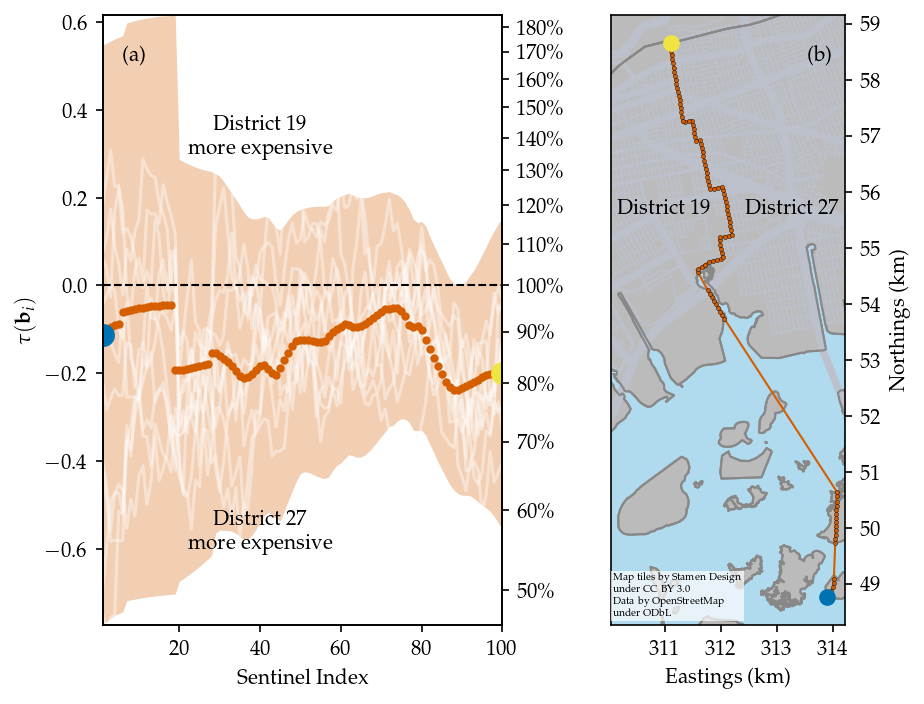
\includegraphics[width=\textwidth]{figures/NYC_cliff_face.png}
  \end{minipage}\hfill
  \begin{minipage}[c]{0.5\textwidth}
    \caption{
        (a)
        Posterior treatment effect \autoref{eq:postvar2gp} for the school district effect on house prices per square foot between district 27 and district 19, with 95\% credible envelope.
        The left \(y\)-axis shows the difference in log prices per square foot; positive values mean prices are higher in district 19.
        The right \(y\)-axis shows the corresponding ratio of the price of a house in district 19 over its price in district 27.
        A few draws from the posterior are shown in lighter color to show the posterior correlations between sentinels.
        (b)
        A map of sentinel locations, evenly spaced along the border between school districts 27 and 19.
    	The southernmost sentinel (shown as a blue circle) has index 1, while the northernmost sentinel (shown in yellow) has index 100.\label{fig:NYC_cliff_height}
    } 
  \end{minipage}
\end{figure}

We illustrate the results with a single pair of neighboring districts: 19 (``treatment'') and 27 (``control'').
We fit the hyperparameters \(\widehat{\sigman}=0.40\), \(\widehat{\sigmaf}=0.26\), \(\widehat{\sigmabeta}=0.15\), and \(\widehat{\ell}=4.9~\text{km}\)
by optimizing the marginal log-likelihood of the data within neighboring school districts 18, 19, 23, 24, 25, 26, 27, 28, and 29,
and set \(\sigmamu=20\) to give the district means \(m_j\) a weak prior.
After fitting the coefficients \(\gamma\) (see \autorefexternal{sec:covariates} in Supplements for details) and extracting residuals, we obtain the posterior treatment effect \autoref{eq:postvar2gp} shown in \autoref{fig:NYC_cliff_height}.

The posterior mean in \autoref{fig:NYC_cliff_height} indicates a negative treatment effect everywhere along the border, which can be averaged by the estimators we developed in \autoref{sec:ate}.
Our two estimators, based on uniform weights and inverse-variance weights, yield LATE estimates (posterior mean \(\pm\) std. deviation) of \(-0.16\pm 0.09\) and \(-0.20 \pm 0.06\) respectively, which corresponds to an approximately 20\% increase in property prices going from district 19 to district 27.
By contrast, treating each district and building class as a fixed effect in an OLS model yields a treatment effect estimate (the difference between the district 19 and 27 coefficients) of -0.12. 

\section{Discussion}

Geographic regression discontinuity designs (GeoRDDs) arise when a treatment is assigned to one region, but not to another adjacent region.
Under smoothness assumptions, units adjacent to the border are comparable, and form a natural experiment.
The same idea underpins causal interpretations of one-dimensional regression discontinuity designs (1D RDDs), where a single ``forcing'' variable controls the treatment assignment.
We use this similarity to motivate a framework for the analysis of GeoRDDs.

We emphasize the importance of the spatial aspect of GeoRDDs, 
using GPR (kriging) to fit smooth surfaces to the outcomes, and to extrapolate to the border.
Our approach yields a multivariate normal posterior on the treatment effect at a set of ``sentinel'' locations along the border.
The use of GPR to analyse GeoRDDs is flexible and presents opportunities for future extensions, 
inspired by developments in spatial statistics and machine learning that are based on Gaussian processes.
For example, if the outcomes are binary, proportions, or counts, then binomial or Poisson likelihoods could be substituted instead of the normal likelihood used in this paper.
We also expect that methodological advances that improve the extrapolating behavior of Gaussian processes \citep[e.g.][]{wilson2013gaussian} would improve the robustness of our method.

Averaging the treatment effect along the border turns out to have surprising pitfalls.
Simply integrating the treatment effect uniformly along the border yields an estimand that is inefficient and undesirably sensitive to the topology of the border.
The inverse-variance weighted estimator is robust to this effect and uses the information available in the data more efficiently.

We applied our method to a publicly available dataset of one year of New York City property sales, to examine whether school district cause difference in property prices.
Focusing on the border between school districts 19 and 27, we estimated an approximately 20\% average increase in house prices per square foot when crossing the border from district 19 to district 27.
However, the border between these two districts is also the border between the NYC boroughs of Brooklyn and Queens, so we cannot attribute this difference to the causal effect of the school districts.
In the Supplements, we extend the GeoRDD analysis to other pairs of adjacent school districts, and find significant effects between many of these pairs.

\newpage
\subsubsection*{Acknowledgments}
This research was supported by the National Science Foundation Graduate Research Fellowship Program under Grant No. 1144152, by the National Science Foundation under Grant No. 1461435, by DARPA under Grant No. FA8750-14-2-0117, by ARO under Grant No. W911NF- 15-1-0172, and by NSERC. Any opinions, findings, and conclusions or recommendations expressed in this material are those of the authors and do not necessarily reflect the views of the National Science Foundation, DARPA, ARO, or NSERC.

\bibliographystyle{alpha}
\bibliography{GeoRDD}

%%%%%%%%%% Merge with supplemental materials %%%%%%%%%%
% https://tex.stackexchange.com/questions/168169/options-for-supplementary-materials-in-preprint-version-revtex-arxiv#169606
\pagebreak
\begin{center}
\phantomsection
	\addcontentsline{toc}{section}{Supplementary Materials}
	\bf 
	\LARGE
	Supplementary Materials
\end{center}
%%%%%%%%%% Merge with supplemental materials %%%%%%%%%%
%%%%%%%%%% Prefix a "S" to all equations, figures, tables and reset the counter %%%%%%%%%%
\setcounter{equation}{0}
\setcounter{figure}{0}
\setcounter{table}{0}
\setcounter{section}{0}
\newcommand{\sprefix}{S-}
\renewcommand{\theequation}{\sprefix\arabic{equation}}
\renewcommand{\thesection}{\sprefix\arabic{section}}
\renewcommand{\thefigure}{\sprefix\arabic{figure}}
\renewcommand{\thetable}{\sprefix\arabic{table}}

\section{Covariances for Gaussian Process Model}
\label{sec:covariances}
All covariances below are conditional on the hyperparameters \(\hyperparam = \del{\ell,\sigmaf, \sigman, \sigmamu}\), omitted for concision.
\begin{equation}
    \begin{split}
        m_\treat, m_\ctrol   &\sim \normal\del{0,\sigmamu^2} \\
        \cov(Y_{i\treat},m_\treat)  &= \cov(Y_{i\ctrol},m_\ctrol) = \sigmamu^2 \\
        \cov(Y_{i\treat},m_\ctrol)  &= \cov(Y_{i\ctrol},m_\treat)  = 0 \\
        \cov\del{Y_{i\treat}, f_{\treat}(\svec')} &= \cov\del{Y_{i\ctrol}, f_{\ctrol}(\svec')} = k(\svec_i,\svec') \\
        \cov\del{Y_{i\treat}, f_{\ctrol}(\svec')} &= \cov\del{Y_{i\ctrol}, f_{\treat}(\svec')} = 0 \\
        \cov(Y_{i\treat},Y_{j\treat}) &= \cov(Y_{i\ctrol},Y_{j\ctrol}) = \sigmamu^2 + k(\svec_i,\svec_j) + \delta_{ij}\sigman^2 \\
        \cov(Y_{i\treat},Y_{j\ctrol}) &= 0
    \end{split}
    \label{eq:covariances}
\end{equation}
We further define some shorthand notation, found in \autoref{table:notation}.

\begin{table}[bp]
    \centering
    \bgroup
    \def\arraystretch{1.2}%  1 is the default, change whatever you need
    \begin{tabular}{lll}
        \hline
        Symbol & Size                       & \(ij^{\mathrm{th}}\) entry                                                      \\ \hline
        \(\KBB\) & \(\numsent \times \numsent\) & \(\sigmamu^2 + k\del{\sentinel_i,\sentinel_j}\)                                 \\ 
        \(\KBT\) & \(\numsent \times n_\treat\) & \(\sigmamu^2 + k\del{\sentinel_i,\svec_{j\treat}}\)                             \\ 
        \(\KBC\) & \(\numsent \times n_\ctrol\) & \(\sigmamu^2 + k\del{\sentinel_i,\svec_{j\ctrol}}\)                             \\
        \(\KTT\) & \(n_\treat \times n_\treat\) & \(\sigmamu^2 + k\del{\svec_{i\ctrol},\svec_{j\ctrol}}\)                         \\
        \(\KCC\) & \(n_\ctrol \times n_\ctrol\) & \(\sigmamu^2 + k\del{\svec_{i\treat},\svec_{j\treat}}\)                         \\ 
        \(\STT\) & \(n_\treat \times n_\treat\) & \(\sigmamu^2 + k\del{\svec_{i\treat},\svec_{j\treat}} + \delta_{ij} \sigman^2\) \\ 
        \(\SCC\) & \(n_\ctrol \times n_\ctrol\) & \(\sigmamu^2 + k\del{\svec_{i\ctrol},\svec_{j\ctrol}} + \delta_{ij} \sigman^2\) \\
        \hline
    \end{tabular}
    \egroup
    \caption{
        Shorthand notation for covariance matrices. The spatial coordinates of the \(i^\mathrm{th}\) treatment unit are denoted by \(\svec_{i\treat}\),
and those of the \(j^\mathrm{th}\) control unit by \(\svec_{j\ctrol}\), while \(\sentinel_i\) denotes the \(i^\mathrm{th}\) sentinel location along the border.
        \label{table:notation}
    }
\end{table}

\section{Handling Nonspatial Covariates}
\label{sec:covariates}

The Gaussian process specification also makes it easy, mathematically and computationally, to incorporate a linear model on nonspatial covariates.
The models are modified by the addition of the linear regression term \(\Xmat \gammavec\) on the \(n \times p\) matrix of covariates \(\Xmat\), where \(p\) is the number of nonspatial covariates.
We recommend placing a normal prior \(\normal(0,\sigmabeta^2)\) on the regression coefficients, as this preserves the multivariate normality of the model, with the simple addition of a term \(\sigmabeta^2 \Xmat \Xmat\trans\) to the covariance \(\SigmaMat_Y\) of \(\Yvec\).
Let \(\xvec_i\) be the \(p\)-vector of nonspatial covariates of unit \(i\).
Our model becomes:
\begin{equation}
    \begin{split}
        & Y_{i\treat} = \underbrace{m_\treat{} + f_\treat{}(\svec_i)}_{g_\treat{}(\svec_i)} + \xvec_i\trans \gammavec + \epsilon_i \quad\text{and}\quad
        Y_{i\ctrol} = \underbrace{m_\ctrol{} + f_\ctrol{}(\svec_i)}_{g_\ctrol{}(\svec_i)} + \xvec_i\trans \gammavec + \epsilon_i \,\text{, with} \\
        & \gamma_j \overset{\indep}{\sim} \normal\del{0,\sigmabeta^2}\,\text{, for }j=1,2,\dotsc,p \,,
    \end{split}
    \label{eq:covariates_model}
\end{equation}
and \(f_\treat\), \(f_\ctrol\) and \(\epsilon_i\) as in \autoref{eq:spec2gp}.

Unfortunately, the linear term induces a covariance between the treatment and control region; \(\SigmaMat_Y\) is no longer black diagonal, which roughly quadruples the computational cost of the analysis, as it requires the inversion of an \((n_\treat{}+n_\ctrol{}) \times (n_\treat{}+n_\ctrol{})\) covariance matrix instead of (in the absence of correlations between the treatment and control units) the separate inversions of the \(n_\treat{} \times n_\treat{}\) covariance matrix \(\STT\), and \(n_\ctrol{} \times n_\ctrol{}\) covariance matrix \(\SCC\).
The introduction of the linear term modifies the cliff height estimator \autoref{eq:postvar2gp} so that its posterior mean and covariance become:
\begin{equation}
    \begin{split}
        \muvec_{\sentinels \mid Y, D} &= 
        \begingroup\SmallColSep
        \begin{bmatrix}
            \KBT & -\KBC
        \end{bmatrix}
        \SigmaMat_Y^{-1}
        \Yvec
        \endgroup
        \,\text{, and}\\
        \Sigma_{\sentinels \mid Y, D} &=
        \begingroup\SmallColSep
        2 \KBB -
        \begin{bmatrix}
            \KBT & -\KBC
        \end{bmatrix}
        \SigmaMat_Y^{-1}
        \begin{bmatrix}
            \KBT & -\KBC
        \end{bmatrix}\trans
        \endgroup
        \,.
    \end{split}
    \label{eq:cliff_with_covariates}
\end{equation}
To avoid the complexity caused by the correlation between \(\yt\) and \(\yc\) that the linear term induces, we suggest first obtaining an estimate \(\hat\gammavec\) of the coefficients:
\begin{equation}
    \begin{split}
        % \Yvec &= \begin{pmatrix}
            % \yt \\
            % \yc
        % \end{pmatrix}
        % \\
        &
        \cov\del{\Yvec \mid \gammavec }
                = \begin{bmatrix}
                    \STT & 0 \\
                    0 & \SCC
                  \end{bmatrix}
            \,,\ 
            \cov\del{\gammavec} = \sigmabeta^2 \eye_p 
            \,,\  
            \cov\del{\Yvec, \gammavec} = \sigmabeta^2 \Xmat \\&
        \SigmaMat_Y = \cov\del{\Yvec} 
            = \cov\del{\Yvec \mid \gammavec}
                + \sigmabeta^2 \Xmat \Xmat\trans \\&
        % &= \begin{bmatrix}
            % \STT\!+\!\sigmabeta^2 \Dmat_{\treat} \Dmat_{\treat}\trans 
            % & \! \sigmabeta^2 \Dmat_{\treat} \Dmat_{\ctrol}\trans \\
            % \sigmabeta^2 \Dmat_{\ctrol} \Dmat_{\treat}\trans 
            % & \! \SCC\!+\!\sigmabeta^2 \Dmat_{\ctrol} \Dmat_{\ctrol}\trans
        % \end{bmatrix}\\
        \hat\gammavec 
            = \E\del{\gamma \mid \Yvec} 
            = \cov\del{\gammavec,\Yvec} \cov\del{\Yvec,\Yvec}^{-1} \Yvec
            = \sigmabeta^2 \Xmat\trans\SigmaMat_{Y}^{-1} \Yvec
        \,.
    \end{split}
\end{equation}
The treatment and control residuals can then be obtained as \(\residvec = \Yvec - \Xmat \hat\gammavec\).
Conditionally on \(\gammavec=\hat\gammavec\), the residuals of the treatment and control units then have independent multivariate normal distributions with covariances \(\STT\) and \(\SCC\) respectively.


We can then proceed with the GeoRDD analysis on the residuals, which are decorrelated conditionally on \(\gammavec=\hat\gammavec\).
This is an approximation, as it ignores the uncertainty in the estimate of \(\gammavec\), but if the number of samples in the treatment and control areas is high (even away from the border), the approximation has negligible effect on the estimate of the treatment effect, and simplifies the subsequent GeoRDD analysis.

%%% NYC %%%
\section{Full Analysis: NYC School Districts}
\label{pairs-of-school-districts}

	The GeoRDD analysis can be repeated for each pair of adjacent districts.
\autoref{fig:NYC_pairwise} and \autoref{table:NYC_pairwise} give an overview of the results by showing the posterior mean and standard deviation of the inverse variance LATE estimated at each border.
Significant effects are found between many districts, but interpreting the results requires some caution.
We have already mentioned the issue of compound treatments for borders between school districts that overlap with the border between boroughs.
School districts 19, 32, and 14 are in Brooklyn, while districts 30, 24, and 27 are in Queens.

\begin{figure}
    \centering
    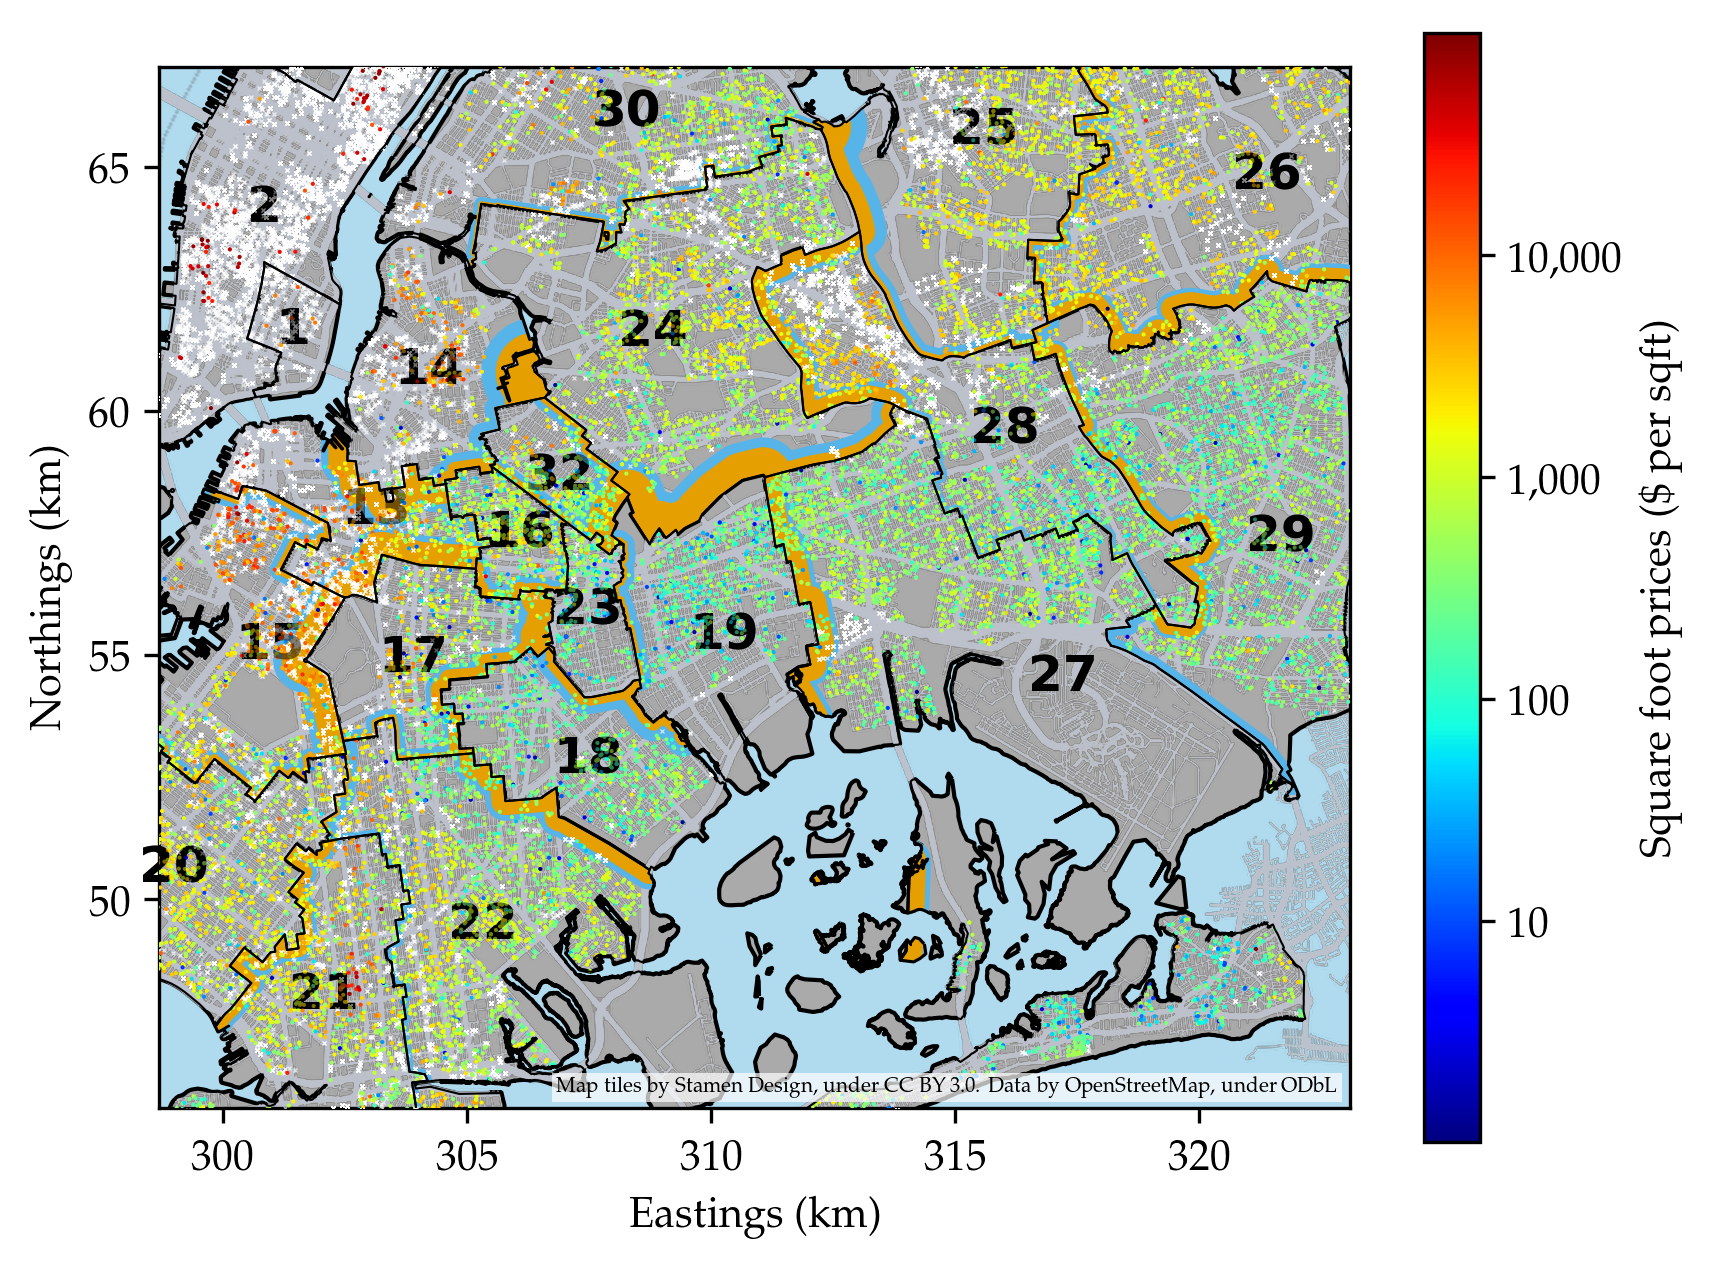
\includegraphics[width=0.97\textwidth,height=0.8\textheight,keepaspectratio]{figures/pairwise_mean_se.pdf}
    \caption[]{
		\label{fig:NYC_pairwise}
        \textbf{Pairwise estimates of the inverse variance LATE between adjacent districts.}
        The thickness of the orange buffer adjacent to borders is proportional to the posterior mean of the inverse variance LATE, and the blue buffer beyond it is proportional to the posterior standard deviation of the LATE.
    The buffers are drawn on the side of the border that is estimated to have higher house prices. 
        \\\hspace{\textwidth}
        \textbf{Background:} 
        Map of property sales in New York City. Each dot is a sale, and its color indicates the price per square foot. White crosses indicate sales of properties with missing square footage, which are therefore excluded from the analysis. School district boundaries are shown, and each district is labeled by its number.
    }
\end{figure}

	Some school districts are separated by parks (or other non-residential zones), for example districts 15 \& 17 or 19 \& 24, so that house sales do not extend all the way to the border on one or both sides.
A significant treatment effect between these pairs cannot be interpreted as the detection of a discontinuity in prices at the border, let alone any kind of causal interpretation, but rather it means that the difference in prices between the two sides of the park exceeds the typical spatial variation of house prices expected over the same distance.
This is not unsurprising, and one may speculate that physical barriers like parks, rivers, railways and major roads can separate neighborhoods with distinct character, demographics and thus house prices.
This in turn challenges the stationarity assumption of the spatial model \autorefexternal{eq:spec2gp}.
The higher distance between data and the border also stretches the spatial model's ability to extrapolate, which makes it more vulnerable to model misspecification.

	Other pairs of district, like 13 \& 14, 13 \& 17, and 25 \& 28 have clusters of missing data (condo sales with unknown square footage) near the border that cast doubt on the interpretation of the estimated effect.
Nonetheless, significant effects are also found between pairs of school districts without issues due to compound treatments, physical barriers, or missing data.
House prices increase going across the border from districts 16 to 13, 18 to 17, 24 to 30, 23 to 17, 25 to 26, 28 to 29, and 29 to 26.
Overall, it seems that school district borders in Brooklyn and Queens can correspond to measurable jumps in house prices per square foot.
The estimated size of this effect varies: zero or negligible in some cases, such as between districts 15, 20, 21, and 22; and quite pronounced in others, such as a 17\% price increase from 29 to 26 and from 18 to 17.

\begin{sidewaystable}
        \footnotesize
        \begin{tabular}{r|lllllll}
            \hline
\( \mathbf{13} \)& \( \mathbf{14:}~-0.30 \pm 0.10 \)& \( \mathbf{15:}~+0.05 \pm 0.08 \)& \( \mathbf{16:}~-0.07 \pm 0.07 \)& \( \mathbf{17:}~-0.16 \pm 0.09 \)\\ 
\( \mathbf{14} \)& \( \mathbf{13:}~+0.30 \pm 0.10 \)& \( \mathbf{16:}~-0.07 \pm 0.12 \)& \( \mathbf{24:}~-0.35 \pm 0.19 \)& \( \mathbf{32:}~-0.04 \pm 0.13 \)\\ 
\( \mathbf{15} \)& \( \mathbf{13:}~-0.05 \pm 0.08 \)& \( \mathbf{17:}~-0.18 \pm 0.11 \)& \( \mathbf{20:}~+0.09 \pm 0.06 \)& \( \mathbf{22:}~+0.40 \pm 0.14 \)\\ 
\( \mathbf{16} \)& \( \mathbf{13:}~+0.07 \pm 0.07 \)& \( \mathbf{14:}~+0.07 \pm 0.12 \)& \( \mathbf{17:}~-0.08 \pm 0.08 \)& \( \mathbf{23:}~-0.10 \pm 0.08 \)& \( \mathbf{32:}~+0.04 \pm 0.08 \)\\ 
\( \mathbf{17} \)& \( \mathbf{13:}~+0.16 \pm 0.09 \)& \( \mathbf{15:}~+0.18 \pm 0.11 \)& \( \mathbf{16:}~+0.08 \pm 0.08 \)& \( \mathbf{18:}~-0.16 \pm 0.07 \)& \( \mathbf{22:}~+0.06 \pm 0.08 \)& \( \mathbf{23:}~-0.29 \pm 0.11 \)\\ 
\( \mathbf{18} \)& \( \mathbf{17:}~+0.16 \pm 0.07 \)& \( \mathbf{19:}~-0.13 \pm 0.14 \)& \( \mathbf{22:}~+0.06 \pm 0.07 \)& \( \mathbf{23:}~-0.08 \pm 0.10 \)\\ 
\( \mathbf{19} \)& \( \mathbf{18:}~+0.13 \pm 0.14 \)& \( \mathbf{23:}~-0.02 \pm 0.09 \)& \( \mathbf{24:}~+0.34 \pm 0.13 \)& \( \mathbf{27:}~+0.20 \pm 0.06 \)& \( \mathbf{32:}~+0.27 \pm 0.15 \)\\ 
\( \mathbf{20} \)& \( \mathbf{15:}~-0.09 \pm 0.06 \)& \( \mathbf{21:}~+0.06 \pm 0.06 \)& \( \mathbf{22:}~-0.08 \pm 0.09 \)\\ 
\( \mathbf{21} \)& \( \mathbf{20:}~-0.06 \pm 0.06 \)& \( \mathbf{22:}~-0.05 \pm 0.05 \)\\ 
\( \mathbf{22} \)& \( \mathbf{15:}~-0.40 \pm 0.14 \)& \( \mathbf{17:}~-0.06 \pm 0.08 \)& \( \mathbf{18:}~-0.06 \pm 0.07 \)& \( \mathbf{20:}~+0.08 \pm 0.09 \)& \( \mathbf{21:}~+0.05 \pm 0.05 \)\\ 
\( \mathbf{23} \)& \( \mathbf{16:}~+0.10 \pm 0.08 \)& \( \mathbf{17:}~+0.29 \pm 0.11 \)& \( \mathbf{18:}~+0.08 \pm 0.10 \)& \( \mathbf{19:}~+0.02 \pm 0.09 \)& \( \mathbf{32:}~-0.07 \pm 0.09 \)\\ 
\( \mathbf{24} \)& \( \mathbf{14:}~+0.35 \pm 0.19 \)& \( \mathbf{19:}~-0.34 \pm 0.13 \)& \( \mathbf{25:}~+0.26 \pm 0.15 \)& \( \mathbf{27:}~-0.17 \pm 0.12 \)& \( \mathbf{28:}~+0.17 \pm 0.07 \)& \( \mathbf{30:}~+0.10 \pm 0.06 \)& \( \mathbf{32:}~-0.01 \pm 0.09 \)\\ 
\( \mathbf{25} \)& \( \mathbf{24:}~-0.26 \pm 0.15 \)& \( \mathbf{26:}~+0.09 \pm 0.05 \)& \( \mathbf{28:}~-0.09 \pm 0.09 \)& \( \mathbf{29:}~+0.06 \pm 0.13 \)& \( \mathbf{30:}~-0.45 \pm 0.22 \)\\ 
\( \mathbf{26} \)& \( \mathbf{25:}~-0.09 \pm 0.05 \)& \( \mathbf{29:}~-0.15 \pm 0.06 \)\\ 
\( \mathbf{27} \)& \( \mathbf{19:}~-0.20 \pm 0.06 \)& \( \mathbf{24:}~+0.17 \pm 0.12 \)& \( \mathbf{28:}~+0.01 \pm 0.04 \)& \( \mathbf{29:}~-0.00 \pm 0.10 \)\\ 
\( \mathbf{28} \)& \( \mathbf{24:}~-0.17 \pm 0.07 \)& \( \mathbf{25:}~+0.09 \pm 0.09 \)& \( \mathbf{27:}~-0.01 \pm 0.04 \)& \( \mathbf{29:}~+0.11 \pm 0.05 \)\\ 
\( \mathbf{29} \)& \( \mathbf{25:}~-0.06 \pm 0.13 \)& \( \mathbf{26:}~+0.15 \pm 0.06 \)& \( \mathbf{27:}~+0.00 \pm 0.10 \)& \( \mathbf{28:}~-0.11 \pm 0.05 \)\\ 
\( \mathbf{30} \)& \( \mathbf{24:}~-0.10 \pm 0.06 \)& \( \mathbf{25:}~+0.45 \pm 0.22 \)\\ 
\( \mathbf{32} \)& \( \mathbf{14:}~+0.04 \pm 0.13 \)& \( \mathbf{16:}~-0.04 \pm 0.08 \)& \( \mathbf{19:}~-0.27 \pm 0.15 \)& \( \mathbf{23:}~+0.07 \pm 0.09 \)& \( \mathbf{24:}~+0.01 \pm 0.09 \)\\ 
            \hline
        \end{tabular}
        \caption{
            \label{table:NYC_pairwise}
            \textbf{Estimated Treatment Effects Between Adjacent NYC School Districts.}
            Each row gives the posterior (mean \(\pm\) standard deviation) of the inverse-variance LATEs for one district (row header) compared to its neighbors.
            For example the first cell indicates an estimated average change in log house prices per square foot of -0.30 when crossing the border from district 13 to 14.
        }
\end{sidewaystable}


\end{document}
